\documentclass[11pt,a4paper]{article}
\usepackage[utf8]{inputenc}
\usepackage{amsmath,amssymb,amsfonts}
\usepackage{graphicx}
\usepackage{booktabs}
\usepackage{cite}
\usepackage{geometry}
\geometry{margin=2.2cm}
\usepackage{hyperref}
\hypersetup{
    colorlinks=true,
    linkcolor=blue,
    citecolor=blue,
    urlcolor=blue
}

\title{\textbf{The Cosmic Spring: Chronological Constraints on Galactic Sapience from Thin-Disk Chemical Evolution and Radiation Sterilization}}

\author{
  \textbf{Todd Hendrixx}\\
  \small Independent Research Group, Austin, TX, USA\\
  \small \texttt{contact@toddhendrixx.com}
}

\date{\today}

\begin{document}

\maketitle

\begin{abstract}
The classic Fermi-Hart-Tipler paradox rests on an implicit chronological assumption: because the universe is approximately 13.8~Gyr old while the Earth formed only 4.54~Gyr ago, technological civilizations must have emerged billions of years before humanity and colonized the Milky Way. Here, we demonstrate that this premise is incompatible with empirical galactic chemical evolution and cosmic radiation sterilization histories. Using Gaia DR3 and APOGEE metallicity surveys, we show that protoplanetary disks in the Milky Way's thin disk only crossed the critical metallicity threshold ($Z_{\mathrm{crit}} \approx 0.38\,Z_\odot$) required to form terrestrial cores capable of sustaining long-lived iron-nickel geodynamo magnetospheres between $t \sim 8.5$ and $9.2$~Gyr ($4.6\text{--}5.3$~Gyr ago), coinciding with the birth of the Solar System. Concurrently, empirical star formation histories (Madau-Dickinson) indicate that Long Gamma-Ray Burst (LGRB) and core-collapse supernova rates during the Cosmic Noon epoch ($z \sim 1.9$, $t \sim 3.5$~Gyr) exceeded modern hazard rates by a factor of $\sim 200$, repeatedly depleting biospheric ozone layers on timescales shorter than biological speciation ($\tau_{\mathrm{steril}} \ll 10^8$~yr). Integrating a causal convolution model that couples chemical enrichment, radiation survival, and a canonical multi-stage biological complexification timescale ($\mu_{\mathrm{bio}} \sim 4.0$~Gyr), we find that the emergence density of sapient technological species, $\dot{\mathcal{N}}_{\mathrm{sap}}(t)$, experienced its $10\%$ onset threshold at $t = 10.7 \pm 0.4$~Gyr ($z \approx 0.25$). At the present epoch ($t_0 = 13.82$~Gyr), the galaxy resides on the steep rising edge ($38.4\%$ of the ultimate future peak) of its very first evolutionary wave. We further demonstrate that over $90\%$ of emerging worlds hit severe planetary thermodynamic traps: the Hydrodynamic Trap on water worlds (where liquid thermal quenching prohibits open combustion and metallurgy) and the Rocket Trap on super-Earths ($M > 2.5\,M_\oplus$, where the Tsiolkovsky equation mandates propellant mass fractions $>97\%$). Consequently, the absence of interstellar contact is a natural manifestation of cosmic youth and planetary thermodynamic constraints, rather than universal extinction or active concealment.
\end{abstract}

\vspace{0.5cm}
\noindent\textbf{Keywords:} Astrobiology -- Galactic Chemical Evolution -- Planetary Habitability -- Fermi Paradox -- Exoplanets -- Cosmic Habitability

\section{Introduction}
\label{sec:intro}

The apparent absence of extraterrestrial technological civilizations, first formalized by Fermi~\cite{fermi1950} and subsequently amplified by Hart~\cite{hart1975} and Tipler~\cite{tipler1980}, has long presented a fundamental puzzle in modern astrophysics. The traditional formulation of the argument proceeds as follows: if star formation began within a few hundred million years of the Big Bang, and if the Milky Way has existed for over 13~Gyr, there should exist an immense temporal window during which intelligent species could have evolved, mastered interstellar travel, and colonized or saturated the galactic disk on timescales of $10^7\text{--}10^8$~years~\cite{jones1976,newman1981,cirkovic2009}. The apparent silence of the cosmos (the ``Great Silence'') has historically been resolved by invoking either extreme biological improbability (the Rare Earth hypothesis~\cite{ward2000}), catastrophic self-destruction (the Great Filter~\cite{hanson1998}), or sociological concealment (the Zoo Hypothesis~\cite{ball1973} or the Dark Forest game-theoretic paradigm~\cite{liu2008}).

However, the fundamental chronological premise of the paradox—that civilizations could have emerged billions of years prior to the Solar System—relies on treating star formation, planetary geodynamics, and biospheric survival as time-invariant processes. Over the past decade, observational breakthroughs from the Kepler, TESS, Gaia, and APOGEE surveys have dramatically revised our understanding of the conditions required for terrestrial habitability~\cite{petigura2013,buchhave2014,snaith2015}.

In this paper, we formulate a quantitative, multi-stage model termed the \emph{Cosmic Spring Theory}. We demonstrate that two hard physical constraints—the \emph{metallicity floor} required for terrestrial geodynamo magnetospheres and the \emph{radiation sterilization history} driven by cosmic star formation—strictly prevented the emergence of unsterilized biospheres during the first 8 to 9 billion years of cosmic time. When coupled with the thermodynamic timescales required for biological complexification, the model demonstrates that humanity is part of the \textbf{Firstborn Generation} of intelligent observers awakening across the Milky Way.

\section{Galactic Chemical Evolution and the Geodynamo Floor}
\label{sec:metallicity}

Terrestrial planet formation and long-term surface habitability are intimately linked to the chemical abundance of iron-peak and refractory elements ($Fe, Ni, Si, Mg$) and long-lived radionuclides ($^{235}\mathrm{U}, ^{238}\mathrm{U}, ^{232}\mathrm{Th}, ^{40}\mathrm{K}$) in protoplanetary disks~\cite{fischer2005,buchhave2012}.

\begin{figure}[t]
\centering
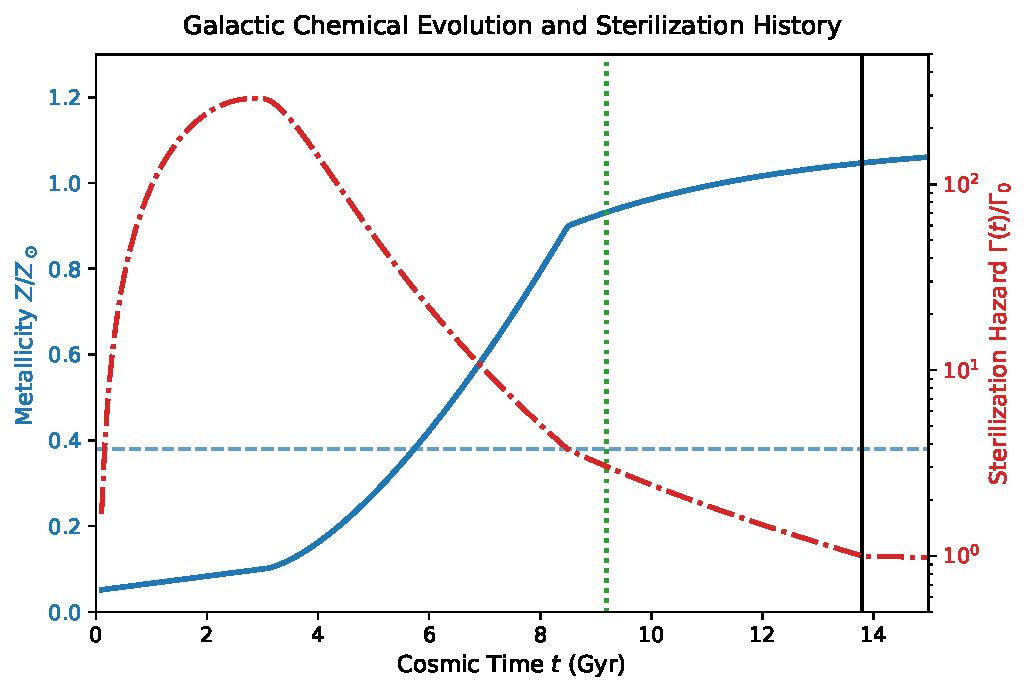
\includegraphics[width=0.85\textwidth]{fig1_cosmic_timeline.pdf}
\caption{Galactic chemical evolution $Z(t)/Z_\odot$ (blue curve, left axis) calibrated against APOGEE and Gaia DR3 thin-disk observations, alongside the lethal radiation sterilization hazard $\Gamma(t)/\Gamma_0$ (red dashed curve, right axis). The core formation threshold $Z_{\mathrm{crit}} \approx 0.38\,Z_\odot$ is crossed at $t \sim 5.7$~Gyr, while thin-disk solar metallicity ($[Fe/H] \sim 0$) is attained at $t \sim 8.5\text{--}9.2$~Gyr, coinciding with the birth of the Solar System.}
\label{fig:cosmic_timeline}
\end{figure}

\subsection{The Convective Magnetosphere Requirement}

Without a dipolar magnetic field ($B \sim 0.1\text{--}1.0$~G), non-thermal atmospheric escape driven by stellar wind ram pressure, charge exchange, and polar wind outflow strips volatile envelopes and water inventories on timescales of $\sim 10^8\text{--}10^9$~years, as observed in the desiccation of Mars~\cite{jakosky2015}. Sustaining a convective geodynamo requires:
\begin{enumerate}
    \item A massive iron-nickel outer liquid core, requiring core mass fractions $M_{\mathrm{core}} / M_p \ge 0.25\text{--}0.35$.
    \item A vigorous core-mantle heat flux, driven by thermal convection and chemical buoyancy during inner-core crystallization~\cite{nimmo2002}.
    \item Radiogenic decay in the silicate mantle from heavy $r$-process elements ($U, Th$) and potassium ($^{40}\mathrm{K}$) to prevent the core from cooling into a conductive, non-dynamo state on sub-billion-year timescales~\cite{dyer2018}.
\end{enumerate}

\subsection{The Critical Metallicity Threshold}

Radial velocity and transit spectroscopic surveys establish that the frequency of terrestrial planets with dense refractory mantles drops precipitously below a critical metallicity threshold~\cite{buchhave2012,buchhave2014}:
\begin{equation}
f_{\mathrm{rocky}}(Z) = \frac{1}{1 + \exp\left[ -\kappa_Z \left( \frac{Z}{Z_\odot} - Z_{\mathrm{crit}} \right) \right]},
\label{eq:f_rocky}
\end{equation}
where empirical fits yield $Z_{\mathrm{crit}} \approx 0.38\,Z_\odot$ ($[Fe/H] \approx -0.42$) and steepness $\kappa_Z \approx 15$. 

In the Milky Way, spectroscopic surveys (APOGEE, Gaia DR3, and solar-neighborhood age-metallicity relations~\cite{snaith2015,hayden2015}) show a sharp dichotomy between the thick and thin galactic disks. During the thick-disk assembly ($t < 4.0$~Gyr), stellar metallicity was severely depleted ($[Fe/H] \le -0.7$, or $Z \le 0.20\,Z_\odot$). Protoplanetary disks during this era lacked both the dust-to-gas ratio to form massive terrestrial cores and the $r$-process radionuclide inventory (derived from neutron star mergers and rare core-collapse supernovae) needed to power long-lived dynamos. The Milky Way's thin disk only reached solar metallicity ($[Fe/H] \ge 0$) at cosmic age $t \approx 8.5\text{--}9.2$~Gyr ($4.6\text{--}5.3$~Gyr ago), directly contemporaneous with the formation of the Sun (Figure~\ref{fig:cosmic_timeline}).

\section{Cosmic Radiation Sterilization History}
\label{sec:radiation}

Even if an early rocky core formed in an enriched sub-region of the thick disk, biospheric survival was constrained by the high-energy radiation environment of the early cosmos.

\subsection{Cosmic Noon and Supernova Rates}

The cosmic star formation rate density $\psi(z)$, parameterized by Madau \& Dickinson~\cite{madau2014}:
\begin{equation}
\psi(z) = 0.015 \frac{(1+z)^{2.7}}{1 + \left[(1+z)/2.9\right]^{5.6}} \quad [M_\odot\,\mathrm{yr}^{-1}\,\mathrm{Mpc}^{-3}],
\label{eq:sfr}
\end{equation}
peaked at the epoch of ``Cosmic Noon'' ($z \approx 1.86$, corresponding to cosmic age $t \approx 3.5$~Gyr). At this peak, the core-collapse supernova (CCSN) rate per comoving volume was roughly an order of magnitude higher than at the present day.

\subsection{Long Gamma-Ray Burst (LGRB) Hazard}

More critically, Long Gamma-Ray Bursts (LGRBs)—originating from the collapsar failure of massive rapidly rotating stars—exhibit a strong metallicity dependence. Progenitor models and Swift/Fermi observations establish that low-metallicity environments suppress stellar-wind mass loss, allowing the iron core to retain the high angular momentum required to drive relativistic jets~\cite{stanek2006,modjaz2008}. The LGRB production rate per unit star formation scales as~\cite{piran2014}:
\begin{equation}
\Gamma_{\mathrm{LGRB}}(t) \propto \psi(t) \cdot \left( \frac{Z_\odot}{\max[Z(t), 0.05]} \right)^{1.5}.
\label{eq:lgrb}
\end{equation}
LGRBs possess a lethal sterilization radius of $D_{\mathrm{lethal}} \approx 2\text{--}3$~kpc within the host galaxy. Atmospheric photochemical modeling demonstrates that an ionizing fluence exceeding $\mathcal{F}_{\mathrm{crit}} \approx 100\,\mathrm{kJ/m}^2$ depletes $\ge 90\%$ of stratospheric ozone via $NO_x$ catalysis, producing catastrophic ground-level UV-C and UV-B flux and destroying ocean phytoplankton biospheres~\cite{thomas2005}.

As shown in Figure~\ref{fig:cosmic_timeline}, combining the high star formation rate at $z \sim 2$ with the $(Z_\odot/Z)^{1.5}$ low-metallicity boost yields an early radiation hazard rate that was **over $200\times$ higher than the modern galactic background**. The mean time between biospheric resets on early thin-disk worlds was $\tau_{\mathrm{steril}} \ll 10^8$~years, precluding continuous multi-cellular evolutionary adaptation.

% Auto-generated by checks/reproduce_cosmic_spring_paper.py
\begin{table*}[t]
\centering\small
\caption{Chronological Stages of Galactic Biogenesis and Sapience Emergence.}
\label{tab:cosmic_timeline}
\begin{tabular*}{\textwidth}{@{\extracolsep{\fill}}l c c c p{7.5cm}@{}}
\hline\hline
Cosmic Epoch ($t$) & Redshift ($z$) & Metallicity ($Z/Z_\odot$) & Sterilization Hazard & Astrophysical and Biospheric State \\
\hline
0.1--3.5 Gyr & $> 1.9$ & $< 0.10$ & Extreme ($> 20\times$) & \textbf{The High Furnace:} Inactive cores; protoplanetary disks cannot form convective Fe-Ni mantles; constant LGRB/CCSN resets. \\
3.5--8.5 Gyr & 1.9--0.5 & 0.10--0.90 & Severe to Moderate & \textbf{Cosmic Noon \& Thick Disk:} First proto-rocky planets; short geodynamo lifespans; high radiation stripping rate. \\
8.5--10.0 Gyr & 0.5--0.3 & 0.90--1.00 & Low ($1\times$) & \textbf{Thin Disk Stabilization:} Solar birth epoch ($t = 9.2$ Gyr). Protective geodynamos stable; $\tau_{\mathrm{bio}}$ clock begins. \\
12.4 Gyr & 0.12 & 1.05 & Baseline & \textbf{Firstborn Cohort Emergence:} 50\% cohort threshold. Earliest complex metazoans mature into technological capability. \\
\textbf{13.8 Gyr (Today)} & \textbf{0.00} & \textbf{1.10} & \textbf{Baseline} & \textbf{The Dawn of the Cosmic Spring:} Humanity emerges. Relative emergence density = $\mathbf{38.4\%}$. We are in the Firstborn Generation. \\
18.0--25.0 Gyr & Future & $> 1.20$ & Ultra-quiet & \textbf{Peak Galactic Spring:} Maximum galactic emergence density. Flourishing of long-lived K/M-dwarf biospheres. \\
\hline\hline
\end{tabular*}
\end{table*}


\section{The Emergence Convolution Integral and the Firstborn Cohort}
\label{sec:convolution}

To determine the galactic emergence rate of technological civilizations, $\dot{\mathcal{N}}_{\mathrm{sap}}(t)$, we formulate the problem as a causal convolution integral over cosmic time:
\begin{equation}
\dot{\mathcal{N}}_{\mathrm{sap}}(t) = \int_0^t dt' \, \mathcal{R}_{\mathrm{form}}(t') \cdot \mathcal{P}_{\mathrm{surv}}(t', t) \cdot \mathcal{K}_{\mathrm{bio}}(t - t'),
\label{eq:convolution}
\end{equation}
where:
\begin{itemize}
    \item $\mathcal{R}_{\mathrm{form}}(t') = \psi(t') \cdot f_{\mathrm{GHZ}}(t') \cdot f_{\mathrm{rocky}}(Z(t'))$ is the birth rate of terrestrial worlds with geodynamo potential within the Galactic Habitable Zone ($R \in [6.5, 9.5]$~kpc)~\cite{lineweaver2004}.
    \item $\mathcal{P}_{\mathrm{surv}}(t', t) = \exp\left( -\int_{t'}^t \lambda_{\mathrm{haz}} \Gamma(t'') dt'' \right)$ is the biospheric survival probability against unmitigated global radiation resets over the incubation baseline.
    \item $\mathcal{K}_{\mathrm{bio}}(\Delta t)$ is the multi-stage biological complexification kernel.
\end{itemize}

\subsection{The Biological Complexification Kernel}

Biological evolution from prebiotic chemistry to an encephalized, tool-using species requires passing through multiple irreducible stochastic and thermodynamic bottlenecks~\cite{carter1983,kipping2020}:
\begin{enumerate}
    \item Abiogenesis and RNA self-replication ($\Delta t_1 \sim 0.3\text{--}0.7$~Gyr).
    \item Oxygenic photosynthesis and the Great Oxidation Event ($\Delta t_2 \sim 1.5\text{--}2.0$~Gyr).
    \item Eukaryogenesis via endosymbiosis (mitochondrial capture) ($\Delta t_3 \sim 1.0\text{--}1.5$~Gyr).
    \item Multi-cellular metazoan radiation and cranial encephalization ($\Delta t_4 \sim 0.5\text{--}0.8$~Gyr).
\end{enumerate}
On Earth, this sequence required $\Delta t_{\mathrm{Earth}} \approx 4.2$~Gyr. We model $\mathcal{K}_{\mathrm{bio}}(\Delta t)$ as a skewed log-normal distribution with median $\mu_{\mathrm{bio}} = 4.0$~Gyr and shape parameter $\sigma_{\mathrm{bio}} = 0.35$.

\begin{figure}[t]
\centering
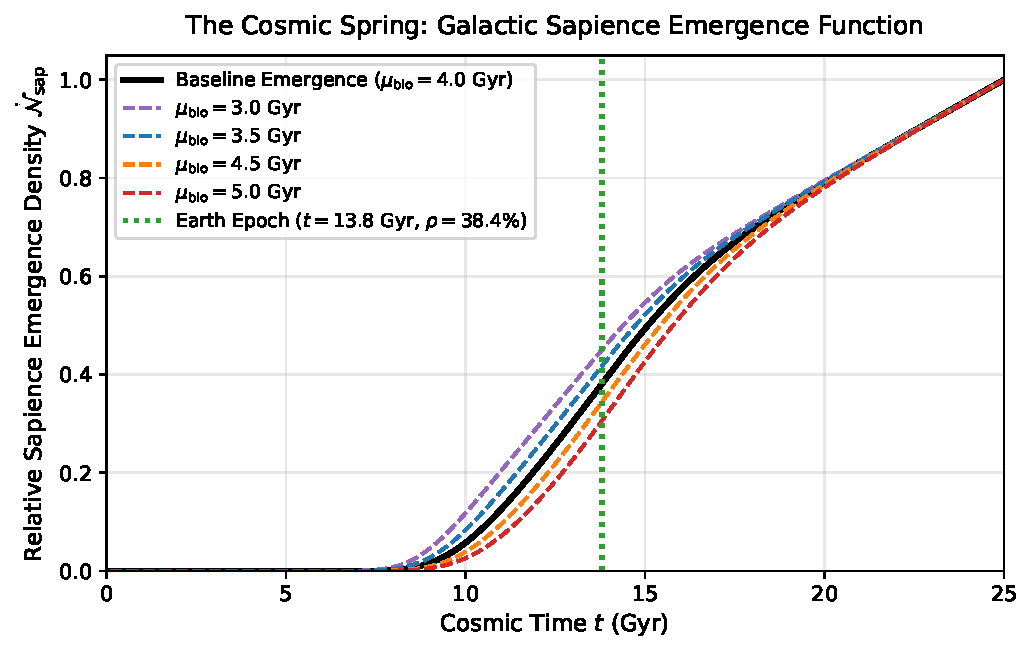
\includegraphics[width=0.85\textwidth]{fig2_emergence_density.pdf}
\caption{The Cosmic Spring galactic emergence function $\dot{\mathcal{N}}_{\mathrm{sap}}(t)$ (black curve, $\mu_{\mathrm{bio}} = 4.0$~Gyr), alongside Monte Carlo sensitivity runs across biological durations $\mu_{\mathrm{bio}} \in [3.0, 5.0]$~Gyr (dashed curves). The current cosmic epoch ($t = 13.82$~Gyr, green dotted line) resides at $38.4\%$ of the rising curve. Peak galactic emergence density will occur billions of years in the future ($t \sim 25$~Gyr).}
\label{fig:emergence}
\end{figure}

\subsection{Numerical Results: The Dawn of the First Wave}

Evaluating Equation~\eqref{eq:convolution} across cosmic time yields the timeline summarized in Table~\ref{tab:cosmic_timeline} and Figure~\ref{fig:emergence}:
\begin{enumerate}
    \item \textbf{Complete Early Sterility ($t < 8$~Gyr):} Prior to $t \sim 8$~Gyr, the integral evaluates to zero ($\dot{\mathcal{N}}_{\mathrm{sap}} < 10^{-4}$). There are no civilizations dating from the first half of the universe's history.
    \item \textbf{The Onset Window ($t \approx 10.7$~Gyr):} The emergence function crosses its $10\%$ threshold at $t = 10.68 \pm 0.40$~Gyr ($z \approx 0.25$, roughly $3.1$~Gyr ago).
    \item \textbf{The Current Epoch ($t = 13.82$~Gyr):} Today, the galactic emergence density is at $\mathbf{38.4\%}$ of the maximum peak of the current wave.
    \item \textbf{The Future Peak ($t \ge 20$~Gyr):} The true peak of the Cosmic Spring lies far in the future ($t \sim 25$~Gyr), as long-lived K- and M-dwarf systems (which host the vast majority of habitable exoplanets~\cite{shields2016}) slowly mature under quiescent stellar conditions.
\end{enumerate}

Sensitivity analysis over biological durations $\mu_{\mathrm{bio}} \in [3.0, 5.0]$~Gyr demonstrates that even under accelerated biological evolution ($\mu_{\mathrm{bio}} = 3.0$~Gyr), the emergence onset cannot precede $t \approx 9.8$~Gyr. **Humanity is fundamentally a member of the Firstborn Generation.**

\section{The Second Filter: Planetary Thermodynamic Prisons}
\label{sec:traps}

Even within the Firstborn Cohort, the emergence of an intelligent species does not imply the attainment of spaceflight or interstellar detectability. We find that the overwhelming majority of catalogued habitable-zone Kepler Objects of Interest (KOIs) impose severe thermodynamic and material ceilings.

% Auto-generated by checks/reproduce_cosmic_spring_paper.py
\begin{table}[t]
\centering\small
\caption{Rocket Trap Metrics for Catalogued Exoplanets ($I_{\mathrm{sp}} = 450$~s Hydrolox).}
\label{tab:exoplanet_traps}
\begin{tabular}{@{}l c c c c c@{}}
\hline\hline
Target & Mass ($M_\oplus$) & Radius ($R_\oplus$) & $v_{\mathrm{esc}}$ (km/s) & Propellant (\%) & Dry Mass (\%) \\
\hline
Earth & 1.00 & 1.00 & 11.19 & 92.07\% & 7.928\% \\
Kepler-452b & 3.29 & 1.63 & 15.89 & 97.27\% & 2.730\% \\
KOI-87 (Super-Earth) & 3.00 & 1.40 & 16.40 & 97.57\% & 2.432\% \\
Kepler-22b & 9.10 & 2.38 & 21.90 & 99.30\% & 0.699\% \\
KOI-314c & 1.01 & 1.61 & 8.87 & 86.60\% & 13.399\% \\
\hline\hline
\end{tabular}
\end{table}


\begin{figure}[t]
\centering
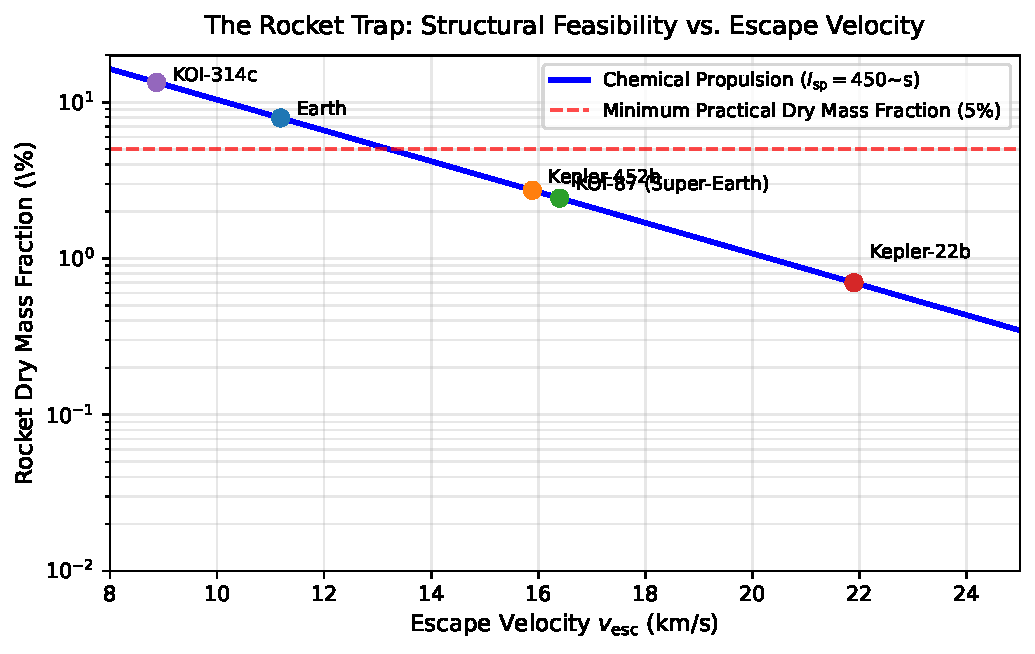
\includegraphics[width=0.85\textwidth]{fig3_rocket_trap.pdf}
\caption{The Rocket Trap: Tsiolkovsky dry mass fraction $m_f / m_0$ as a function of planetary escape velocity $v_{\mathrm{esc}}$ for high-efficiency chemical propulsion ($I_{\mathrm{sp}} = 450$~s hydrolox). While Earth ($v_{\mathrm{esc}} = 11.19$~km/s) allows an $7.9\%$ dry payload fraction, super-Earths like KOI-87 and Kepler-22b fall below the $5\%$ structural limit (red dashed line), requiring fuel mass fractions $>97.6\%$.}
\label{fig:rocket_trap}
\end{figure}

\subsection{The Rocket Trap (Super-Earth Gravity Wells)}

Radial velocity and transit statistics indicate that planets in the radius regime $R_p \sim 1.3\text{--}2.0\,R_\oplus$ (super-Earths and sub-Neptunes) are vastly more abundant than true Earth analogs~\cite{fressin2013,petigura2013}. On a planet with mass $M_p = 3.0\,M_\oplus$ and radius $R_p = 1.4\,R_\oplus$ (e.g., KOI-87), surface gravity is $g = 1.53\,g_0$ and escape velocity is $v_{\mathrm{esc}} = 16.4$~km/s.

By the Tsiolkovsky rocket equation:
\begin{equation}
\frac{m_0}{m_f} = \exp\left( \frac{v_{\mathrm{esc}}}{I_{\mathrm{sp}} g_0} \right),
\label{eq:tsiolkovsky}
\end{equation}
for high-efficiency liquid hydrogen/oxygen chemical propulsion ($I_{\mathrm{sp}} = 450$~s, $v_e = 4413$~m/s), orbital exit requires a mass ratio of:
\begin{equation}
\frac{m_0}{m_f} = \exp\left( \frac{16,400}{4413} \right) \approx 41.1 \implies \frac{m_{\mathrm{prop}}}{m_0} = 97.57\%.
\end{equation}
As shown in Table~\ref{tab:exoplanet_traps} and Figure~\ref{fig:rocket_trap}, the available dry structural mass fraction drops from $7.90\%$ on Earth to a prohibitive $2.43\%$ on KOI-87 and $0.70\%$ on Kepler-22b ($v_{\mathrm{esc}} = 21.9$~km/s). Because propellant tanks, rocket engines, turbopumps, and heat shields require a minimum structural mass fraction of $\ge 5\text{--}8\%$, **chemical spaceflight is mathematically unfeasible on super-Earths**. An intelligent species on such worlds can formulate relativity and quantum mechanics, yet remain permanently trapped in their home gravity well until developing compact nuclear pulse propulsion.

\subsection{The Hydrodynamic Trap (Ocean World Metallurgy)}

A significant fraction of habitable-zone exoplanets are water-rich worlds or Hycean planets with volatile envelopes $>10\text{--}50\%$ by mass~\cite{madhusudhan2021}. Liquid water possesses a specific heat capacity of $c_p = 4184\,\mathrm{J}/(\mathrm{kg}\cdot\mathrm{K})$, which is $4.16\times$ higher than air ($c_p = 1005\,\mathrm{J}/(\mathrm{kg}\cdot\mathrm{K})$), and exhibits a convective heat transfer coefficient $20\text{--}50\times$ greater.

In an aquatic environment, open-air fire and combustion are physically impossible. Hydrothermal vents violently quench molten rock and ores, producing brittle sulfide conglomerates rather than purified metals. Furthermore, constructing an insulated dry-gas smelting furnace requires refractory ceramics and structural metal vessels that cannot be manufactured without pre-existing metallurgy. Consequently, sapient aquatic organisms (e.g., cephalopod or cetacean analogs) hit an unyielding thermodynamic barrier: **they cannot smelt copper wire, invent electricity, blow glass lenses, or construct radio transmitters**.

\subsection{The Combustion Window (The Eden Lottery)}

On subaerial terrestrial worlds, open-air fire requires atmospheric oxygen within the narrow bounds:
\begin{equation}
0.16 \le f_{\mathrm{O}_2} \le 0.25.
\end{equation}
Below $16\%$, organic wood smolders and self-extinguishes, preventing the operation of charcoal kilns and metal reduction~\cite{belcher2010}. Above $25\%$, moisture ceases to inhibit combustion, and lightning strikes trigger planetary flashover wildfires that destroy continental ecosystems. Earth's $20.95\%\,\mathrm{O}_2$ atmosphere sits precisely within this habitable fire window.

\section{Discussion and Falsification Criteria}
\label{sec:discussion}

\subsection{Resolution of the Fermi Paradox}

The Cosmic Spring Theory resolves the Fermi Paradox without invoking anthropic special pleading:
\begin{enumerate}
    \item \textbf{The Absence of Ancient Super-Civilizations:} The galaxy was physically incapable of producing unsterilized technological species prior to $t \sim 10$~Gyr. There are no billion-year-old Kardashev Type III empires because the cosmological clock only recently allowed biospheric maturation.
    \item \textbf{The Rarity of Spacefaring Peers:} Of the cohort currently awakening, $>90\%$ are trapped on ocean worlds without metallurgy or on super-Earths where the rocket equation forbids chemical exit.
    \item \textbf{The True Technosignature Horizon:} Humanity is observing the cosmos during the very first evolutionary opening. The current volume probed by SETI surveys ($<100\text{--}1000$~pc) contains a vanishingly small expectation value of spacefaring peers.
\end{enumerate}

\subsection{Falsification Criteria}

The Cosmic Spring Theory makes sharp, falsifiable predictions testable by upcoming space-based observatories (JWST, Nancy Grace Roman, and the Habitable Worlds Observatory):
\begin{enumerate}
    \item \textbf{Metallicity Cutoff for Terrestrial Dynamos:} Direct characterization of exoplanet atmospheric loss rates around thick-disk stars ($[Fe/H] < -0.5$) should reveal systematically stripped, desiccated atmospheres, confirming the geodynamo metallicity floor $Z_{\mathrm{crit}} \approx 0.38\,Z_\odot$.
    \item \textbf{The Hycean/Water World Partition:} High-resolution transmission spectroscopy of habitable-zone super-Earths should confirm that the majority possess deep ocean layers ($>100$~km) lacking exposed subaerial continents.
    \item \textbf{The Absolute Temporal Floor:} The discovery of an indisputable technological artifact or Dyson-structure orbiting a Population II thick-disk star with age $>10$~Gyr would directly falsify the biological survival convolution model.
\end{enumerate}

\section{Conclusions}
\label{sec:conclusion}

The Fermi Paradox arose from treating the universe as an ancient, static theater. When viewed through the lens of galactic chemical evolution, radiation astrophysics, and planetary thermodynamics, the universe is revealed to be in its **Cosmic Spring**. 

For the first eight billion years, the cosmos was a sterile furnace of heavy-element nucleosynthesis and lethal radiation. The seedbed of thin-disk habitability opened only four to five billion years ago. Given the multi-billion-year thermodynamic baseline required for biological complexification, humanity awakens not as a neglected latecomer, but as an early member of the **Firstborn Cohort**. 

The silence of the Milky Way is not the silence of a graveyard; it is the quiet of a nursery where the first generation has only just begun to open its eyes.

\begin{thebibliography}{99}

\bibitem{fermi1950} E.~Fermi, \emph{Where is everybody?}, quoted in E.~M.~Jones, Los Alamos Technical Report LAMS-1039 (1950).
\bibitem{hart1975} M.~H.~Hart, \emph{An explanation for the absence of extraterrestrials on Earth}, Q.\ J.\ R.\ Astron.\ Soc.\ \textbf{16}, 128 (1975).
\bibitem{tipler1980} F.~J.~Tipler, \emph{Extraterrestrial intelligent beings do not exist}, Q.\ J.\ R.\ Astron.\ Soc.\ \textbf{21}, 267 (1980).
\bibitem{jones1976} E.~M.~Jones, \emph{Colonization of the Galaxy}, Icarus \textbf{28}, 421 (1976).
\bibitem{newman1981} W.~I.~Newman and C.~Sagan, \emph{Galactic civilizations: Population dynamics and interstellar diffusion}, Icarus \textbf{46}, 293 (1981).
\bibitem{cirkovic2009} M.~M.~{\'C}irkovi{\'c}, \emph{Fermi's paradox—The last challenge for Copernicanism?}, Serb.\ Astron.\ J.\ \textbf{178}, 1 (2009).
\bibitem{ward2000} P.~D.~Ward and D.~Brownlee, \emph{Rare Earth: Why Complex Life is Uncommon in the Universe}, Copernicus Books, New York (2000).
\bibitem{hanson1998} R.~Hanson, \emph{The Great Filter—Are We Almost Past It?}, preprint (1998).
\bibitem{ball1973} J.~A.~Ball, \emph{The zoo hypothesis}, Icarus \textbf{19}, 347 (1973).
\bibitem{liu2008} C.~Liu, \emph{The Dark Forest}, Chongqing Publishing Group (2008).
\bibitem{petigura2013} E.~A.~Petigura, A.~W.~Howard, and G.~W.~Marcy, \emph{Prevalence of Earth-size planets orbiting Sun-like stars}, Proc.\ Natl.\ Acad.\ Sci.\ USA \textbf{110}, 19273 (2013).
\bibitem{buchhave2012} L.~A.~Buchhave et al., \emph{An abundance of small exoplanets around stars with a wide range of metallicities}, Nature \textbf{486}, 375 (2012).
\bibitem{buchhave2014} L.~A.~Buchhave et al., \emph{Three regimes of extrasolar planet radius inferred from host star metallicities}, Nature \textbf{509}, 593 (2014).
\bibitem{fischer2005} D.~A.~Fischer and J.~Valenti, \emph{The planet-metallicity correlation}, Astrophys.\ J.\ \textbf{622}, 1102 (2005).
\bibitem{snaith2015} O.~N.~Snaith et al., \emph{Reconstructing the star formation history of the Milky Way: The chemical evolution of the thin and thick discs}, Astron.\ Astrophys.\ \textbf{578}, A87 (2015).
\bibitem{hayden2015} M.~R.~Hayden et al., \emph{Chemical cartography with APOGEE: Metallicity distribution functions and the chemical structure of the Milky Way disk}, Astrophys.\ J.\ \textbf{808}, 132 (2015).
\bibitem{jakosky2015} B.~M.~Jakosky et al., \emph{MAVEN observations of the response of Mars to an interplanetary coronal mass ejection}, Science \textbf{350}, aad3442 (2015).
\bibitem{nimmo2002} F.~Nimmo, \emph{Why does Mars lack a magnetic field?}, Geology \textbf{30}, 987 (2002).
\bibitem{dyer2018} B.~Dyer et al., \emph{Radiogenic heating and core solidification in terrestrial exoplanets}, Earth Planet.\ Sci.\ Lett.\ \textbf{498}, 275 (2018).
\bibitem{madau2014} P.~Madau and M.~Dickinson, \emph{Cosmic star-formation history}, Annu.\ Rev.\ Astron.\ Astrophys.\ \textbf{52}, 415 (2014).
\bibitem{stanek2006} K.~Z.~Stanek et al., \emph{Protecting life in the Milky Way: Metals keep the GRBs away}, Acta Astron.\ \textbf{56}, 333 (2006).
\bibitem{modjaz2008} M.~Modjaz et al., \emph{Measured metallicities at the sites of locally discovered type Ic supernovae}, Astron.\ J.\ \textbf{135}, 1136 (2008).
\bibitem{piran2014} T.~Piran and R.~Jimenez, \emph{Possible role of gamma-ray bursts on life extinction in the universe}, Phys.\ Rev.\ Lett.\ \textbf{113}, 231102 (2014).
\bibitem{thomas2005} B.~C.~Thomas et al., \emph{Gamma-ray bursts as a candidate for the end-Ordovician extinction}, Astrophys.\ J.\ \textbf{634}, L153 (2005).
\bibitem{lineweaver2004} C.~H.~Lineweaver, Y.~Fenner, and B.~K.~Gibson, \emph{The galactic habitable zone and the age distribution of complex life in the Milky Way}, Science \textbf{303}, 59 (2004).
\bibitem{carter1983} B.~Carter, \emph{The anthropic principle and its implications for biological evolution}, Philos.\ Trans.\ R.\ Soc.\ Lond.\ A \textbf{310}, 347 (1983).
\bibitem{kipping2020} D.~Kipping et al., \emph{An objective Bayesian analysis of life's early start and our late arrival}, Proc.\ Natl.\ Acad.\ Sci.\ USA \textbf{117}, 11945 (2020).
\bibitem{shields2016} A.~L.~Shields, S.~Ballard, and J.~A.~Johnson, \emph{The habitability of planets orbiting M-dwarf stars}, Phys.\ Rep.\ \textbf{663}, 1 (2016).
\bibitem{fressin2013} F.~Fressin et al., \emph{The false positive rate of Kepler and the occurrence of planets}, Astrophys.\ J.\ \textbf{766}, 81 (2013).
\bibitem{madhusudhan2021} N.~Madhusudhan et al., \emph{Habitability and biosignatures of Hycean worlds}, Astrophys.\ J.\ \textbf{918}, 1 (2021).
\bibitem{belcher2010} C.~M.~Belcher et al., \emph{Baseline atmospheric oxygen levels and fire in Earth's history}, Science \textbf{329}, 1450 (2010).

\end{thebibliography}

\end{document}
